% ----------------------- TODO ---------------------------
% Diese Daten müssen pro Blatt angepasst werden:
\newcommand{\NUMBER}{1}
\newcommand{\EXERCISES}{5}
% Diese Daten müssen einmalig pro Vorlesung angepasst werden:
\newcommand{\COURSE}{HPC Lab - Assignment 1}

\newcommand{\STUDENTA}{Zirong Cai}
\newcommand{\STUDENTB}{Phuong Nguyen}
\title{\vspace{-2em} Assignment 1 - SIMD \vspace{-0.5em}}
\author{ \STUDENTA, \STUDENTB}
\date{\today {\vspace{-1cm}}}

% ----------------------- TODO ---------------------------

\documentclass[article]{scrartcl}

\usepackage[utf8]{inputenc}
\usepackage[ngerman]{babel}
\usepackage{amsmath}
\usepackage{amssymb}
\usepackage{fancyhdr}
\usepackage{color}
\usepackage{graphicx}
\usepackage{lastpage}
\usepackage{listings}
\usepackage{tikz}
\usepackage{pdflscape}
\usepackage{subfigure}
\usepackage{float}
\usepackage{polynom}
\usepackage{hyperref}
\usepackage{tabularx}
\usepackage{forloop}
\usepackage{geometry}
\usepackage{listings}
\usepackage{caption}
\usepackage{fancybox}
\usepackage{tikz}
\usepackage{algpseudocode,algorithm,algorithmicx}
%\usepackage{biblatex}
\usepackage{cite}

\setkomafont{title}{\normalsize}
\setkomafont{author}{\small}
\setkomafont{date}{\small}
\setkomafont{section}{\normalfont \normalsize \textbf}
\setkomafont{subsection}{\normalfont}
\renewcommand*{\thesubsection}{\alph{subsection}}

\setkomafont{subsubsection}{\normalfont\itshape}

\lstset { %
    language=C++,
    backgroundcolor=\color{black!5}, % set backgroundcolor
    basicstyle=\footnotesize,% basic font setting
}
%\captionsetup[lstlisting]{ format=listings, labelfont=white, textfont=white}

%Definiere Let-Command für algorithmen
%\newcommand*\Let[2]{\State #1 $\gets$ #2}

%\input kvmacros

%Größe der Ränder setzen
\geometry{a4paper,left=3cm, right=3cm, top=3cm, bottom=3cm}

%Kopf- und Fußzeile
\pagestyle {fancy}
\fancyhead[L]{\STUDENTA, \STUDENTB}
\fancyhead[R]{\COURSE}

\fancyfoot[L]{}
\fancyfoot[R]{Page \thepage /\pageref*{LastPage}}

\begin{document}


\maketitle
\thispagestyle{fancy}

\section{CoolMUC2 warm-up}
\subsection{What is the module system and how do you use it?}
According to \cite{modulesys}, The module system is a concept available on most supercomputers, simplifying the use of different software (versions) in a precise and controlled manner.
In most cases, a supercomputer has far more software installed than the average user will ever use. Each of these software packages need different settings in terms of \$PATH, \$LD\_LIBRARY\_PATH and other environment variables, which can adversely affect each other or even be mutually exclusive. Secondly, different user (groups) need different versions of the same software, which in general cannot be installed nor used in parallel on the same system.\\\\
How to use: use \textbf{module} command.

\subsection{What are the following terms: TORQUE, SLURM, and LoadLeveler? What is common
between them?}
\begin{itemize}
    \item TORQUE: TORQUE is a resource manager providing control over batch jobs and distributed compute nodes.
    \item SLURM: The Slurm Workload Manager, formerly known as Simple Linux Utility for Resource Management (SLURM), or simply Slurm, is a free and open-source job scheduler for Linux and Unix-like kernels
    \item LoadLeveler: LoadLeveler is a job management system that allows users to run more jobs in less time by matching the jobs' processing needs with the available resources.
\end{itemize}
\subsection{How can you execute programs on the cluster’s compute nodes? Describe the interactive mode and the batch mode.}
All parallel programs in the parallel segments of the cluster must be started up using either
\begin{itemize}
    \item an interactive SLURM shell: For performing program testing and short runs, accessed via salloc, srun, etc. command
    \item a SLURM batch script: used for all production runs, accessed by writing a script and submit it.
\end{itemize}
\subsection{What software is installed on the Linux-Cluster to manage workload and resources of
multiple users?}
\begin{itemize}
    \item SLURM
\end{itemize}

\subsection{Let’s consider the batch mode. Write a simple “hello world” program which prints the
host-name of the current machine.
Compile the program and write a batch script ([9], [10]) which runs your program
on 2 different nodes of the CoolMUC2 cluster. (In parallel, do not just execute the
batch script twice.) Inspect logs and check that, indeed, two different host-names were
printed.
Include the source code, batch script, and log in your submission.}
\begin{lstlisting}[frame=single]
Code:
#include <stdio.h>
#include <stdlib.h>
#include <unistd.h>

int main()
{
    char hostbuffer[256];
    int hostname;

    // To retrieve hostname
    hostname = gethostname(hostbuffer, sizeof(hostbuffer));

    printf("Hostname: %s\n", hostbuffer);

    return 0;
}
\end{lstlisting}
\begin{lstlisting}[frame=single]
Batch script:
#!/bin/bash
#SBATCH -J hello_host
#SBATCH -o ./%x.%j.%N.out
#SBATCH -D ./
#SBATCH --get-user-env
#SBATCH --clusters=cm2_tiny
#SBATCH --partition=cm2_tiny
#SBATCH --nodes=2
#SBATCH --ntasks-per-node=1
#SBATCH --mail-type=end
#SBATCH --export=NONE
#SBATCH --time=00:02:00
  
module load slurm_setup

echo "Running Program"
mpiexec -n $SLURM_NTASKS ./hello_host
--------------------------------------
Output:
Running Program
Hostname: i23r02c06s08
Hostname: i23r02c06s09

\end{lstlisting}

\section{Auto-vectorisation (2P)}

\subsection{Why is it important to align data structures?}
At each address there is a byte which can be accessed individually. But words can only be fetched at even addresses. So if we read a word at 0000, we read the bytes at 0000 and 0001. But if we want to read the word at position 0001, we need two read accesses. First 0000,0001 and then 0002,0003 and we only keep 0001,0002. And this process take extra time. Aligning data makes accessing data faster.
\subsection{Which kinds of obstacles can prevent vectorisation?}
\begin{itemize}
    \item Non-contiguous memory access
    \item Data dependencies
\end{itemize}
\subsection{Is there a way to assist the compiler through language extensions? If yes, please give details.}
Yes. One can assists the compiler through language extensions, for example from $malloc.h$ extension, one can initialize data with given desired alignment by the function $\_\_mm\_malloc()$. Besides, to tell the compiler that a data is aligned, one can use $\_\_assume\_aligned()$. Then the compiler knows that the accessing data is aligned and can access more effectively. \\

Another way to assist compilers for vectorisation is using C preprocessor - $\#pragma$ directives. Even though it's not a language extension, it's worth to be mentioned here. With $\#pragma$ directives, one can give compilers additional information, for example point out that the loop is vectorizable and no data dependencies which is not recognized by the compiler itself (sometimes).
\subsection{Which loop optimisations are performed by the compiler in order to vectorise and
pipeline loops?}
\begin{itemize}
  \item Loop interchange: For nested loop, compilers can perform optimisations through exchanging the order of two iteration variables. The variables used in the inner loop switch to outer loop, and vice versa. By this, the program has better memory access pattern.
  \item Loop unrolling: compilers interpreting the iterations into a sequence of instructions. This helps to reduce the loop control instructions, reduce miss branch penalties, and hide latencies especially the latencies of reading data from the memory.
\end{itemize}

\section{Vectorisation of 2D image convolution using AVX2Intel Intrinsics (3P + (1P + 2P))}
\subsection{ Theoretical speed up }
Since AVX2 can caculate 8 float point values in one time, the theoretical speed up should be 8.

\subsection{ Optimisation Strategy }
Inspired from \cite{8310675}, We parallelize the algorithm as showed in the picture \ref{fig:2D_strategy} below.

\begin{figure}[htpb]
    \centering
    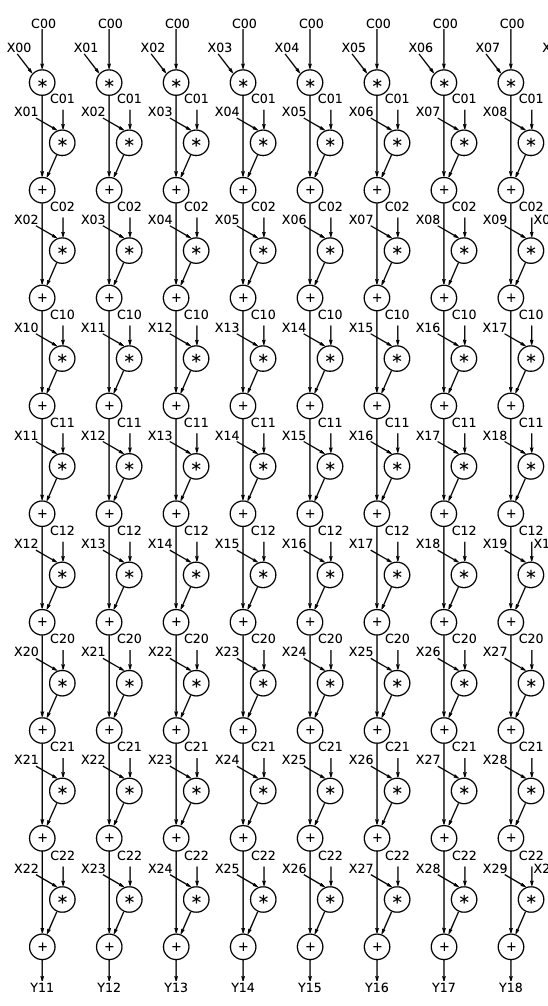
\includegraphics[width=\textwidth,height=6cm,keepaspectratio=true]{../figs/2D_strategy.png}
    \caption{Data flow graph of vectorization of 2-D convolution kernel for an
    3x3 window size using broadcasting of coefficients into a vector register
    and multiply them with image pixels\cite{8310675}.}
    \label{fig:2D_strategy}
\end{figure}


\begin{lstlisting}[frame=single]
__m256 C[k_total_size]; // filter coefficinet vector
__m256 I[k_total_size]; // image data vector
__m256 tmp[k_total_size];
__m256 result = _mm256_setzero_ps();
int i = 0;
for (int yy = -k_half_height; yy <= k_half_height; ++yy)
{
    for (int xx = -k_half_width; xx <= k_half_width; ++xx)
    {
        //broadcast the filter coefficient to a YMM register
        C[i] = _mm256_set1_ps(filter_data[filter.get_rel_index(xx, yy)]);
        //load input data into YMM register
        I[i] = _mm256_load_ps(
        inputdata[channel][input.get_index(x + xx, y + yy)]);
        //AVX multiplication
        tmp[i] = _mm256_mul_ps(C[i], I[i]);
        i++;
    }
}

for (int i = 0; i < k_total_size; ++i)
{
    result = _mm256_add_ps(result, tmp[i]);
}
\end{lstlisting}

\subsection{ data alignment }

The input data may not always be aligned, so
\begin{itemize}
    \item Either use the \textbf{ \_mm256\_loadu\_ps } instruction which can handle the unaligned data
    \item Or use \textbf{\_\_attribute\_\_((aligned(64)))} to force the data to be aligned and then use the \textbf{\_mm256\_load\_ps}
\end{itemize}

\subsection{result}
\begin{center}
\begin{tabular}{ |c|c| } 
 \hline
 kernel width: 3 & kernel width: 3\\ 
 kernel height: 3 &  kernel height: 3\\
 num repeats: 100 & num repeats: 100 \\ 
 mode: default & mode: intrinsics\\
 time spent: 1.34737 sec & time spent: 0.39526 sec\\
 \hline
\end{tabular}
\end{center}
The achieved speed up is:
$$ speedup = \frac{native \ code}{simd \ implementation} = \frac{1.34737 \ sec}{0.39526 \ sec} = 3.40882$$

\subsection{option: Gauss Elimination vectorized with intrinsics}
The first step of Gauss Elimination is called \textbf{Forward Elimination}, below is an example of Forward Elimination:
\begin{figure}[htpb]
    \centering
    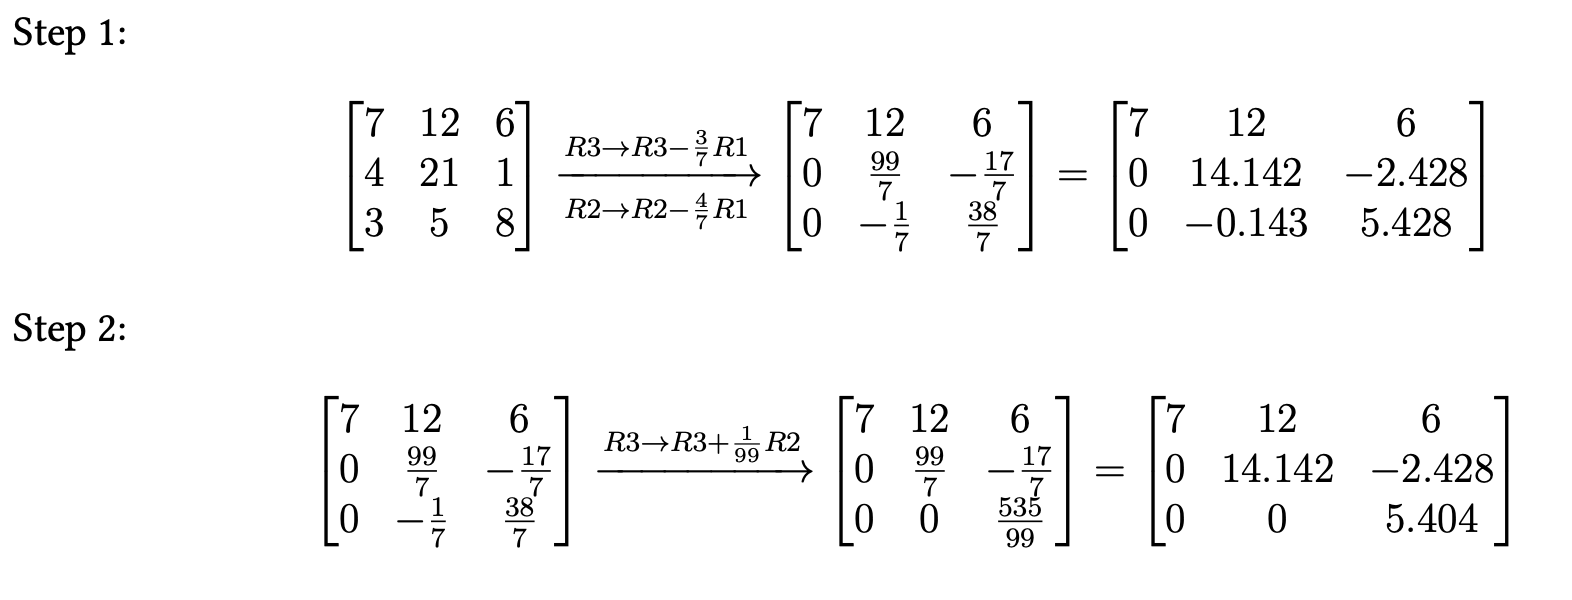
\includegraphics[width=\textwidth,height=6cm,keepaspectratio=true]{../figs/Gauss_Elimination.png}
    \label{fig:Gauss_Elimination}
\end{figure}

We can now formally define the algorithm with simd as follows:
\begin{lstlisting}[frame=single]
for k = 1 to n-1 do
    for i  = k+1 to n do
        a[i][k]] = a[i][k] / a[k][k];
        for each 8 j = k + 1 to n do //implement simd here in this loop
            a[i][j] = a[i][j] - a[i][k] * a[k][j]];
        end
        b[i] = b[i] - a[i][k]*b[k]
    end
end    
\end{lstlisting}
Likewise we can vectorize the second step of Gauss Elimination called Backward Substitution.

\section{ The perfect DGEMM micro-kernel (4P)}
\subsection{System information}
\begin{itemize}
  \item CPU Model: Intel(R) Xeon(R) CPU E5-2697 v3 @ 2.60GHz
  \item Caches: L1d: 32K, L1i: 32K, L2: 256K, L3: 17920K
\end{itemize}


\subsection{Theoretical Performance of a single core}
According to \cite{haswell16} and \cite{haswell}, E5-2697v3 has AVX2 and 2 x FMA instruction. Thus the Theoretical performance of a single core is: \\
$$ P_{peak} = (2.60 GHz) x (4*2*2  FLOPs/cycle) = 41.6 GFLOPs $$

\subsection{Optimisation Strategy}

In this tasks, we are going to optimize the DGEMM. The naive implentation is given as follows:
\begin{lstlisting}[frame=single]
void dgemm(double* A, double* B, double* C) {
    for (int n = 0; n < N; ++n) {
        for (int m = 0; m < M; ++m) {
            for (int k = 0; k < K; ++k) {
                C[n*M + m] += A[k*M + m] * B[n*K + k];
            }
        }
    }
}
\end{lstlisting}

We will first discuss about one simple optimisation which is implement in $kerner2.cpp$, following by the optimisation which was described in the paper \cite{Goto08} and implemented in $kernel1.cpp$.

\subsubsection{Implementation 1}
This is a simple, obvious optimisation stragegy which we found out through analyzing the naive implementation, including:
\begin{itemize}
	\item Loop order interchange: The original order was $N-M-K$. With this order, reading A, B, C are not contiguous in the most inner loop. Reording it to $N-K-M$ gives the function a better memory access pattern, in which both data accessing respecting to A and C are contiguous, while B(n,k) does not depend on the iteration in the M-loop.
	\item Re-using values of B(n,k): After loop order is altered to $N-K-M$, B(n,k) value does not depend on iterations in the M-loop, thus one can use a temporary variable to store value of B(n,k) before the M-loop, and reused it in the M-loop. 
	\item Data alignment to assist vectorisation: According to \cite{align13}, memory movement is optimal when the data starting address lies on 64 byte boundaries. To have this, besides aligning data at the inializing step, one also need to tell the compiler (especially when accessing data in an called function), that given data is aligned. For this, we use $\_\_assume\_aligned(A,64)$.
	\item Blocking: The matrices are splitted into submatrix with the idea that accessing data can stay in caches, and can be re-used as much as possible. With this, we have less caches misses, and less data movement from memory to caches.
	\item Loop unrolling: By default, the loop is unrolled by a factor of 8 by the compiler. We also tested with loop unrolling manually, with a unrolling factor of 4, 8, and 16, but the performance is not better then the default one. Thus, we decided to keep the default unrolling with compiler, rather than the manual unrolling implentation. 
\end{itemize} 
This is the final implementation for this optimisation stragegy:
\begin{lstlisting}[frame=single]
void dgemm_opt(double* A, double* B, double* C) {

    __assume_aligned(A, ALIGNMENT);
    __assume_aligned(B, ALIGNMENT);
    __assume_aligned(C, ALIGNMENT);

    int ii, kk, jj, m, n, k, B_reused;

    for(n = 0; n < N; n += BLOCK_SIZE){
        for(k = 0; k < K; k += BLOCK_SIZE){
            for(m = 0; m < M; m += BLOCK_SIZE){
                for(jj = n; jj < n+BLOCK_SIZE; jj++){
                    for(kk = k; kk < k+BLOCK_SIZE; kk++){
                        B_reused = B[jj*K+kk];
                        for(ii = m; ii < m+BLOCK_SIZE; ii++){
                            //A_reused = A[K*ii+jj];
                            C[jj*M+ii] += A[kk*M+ii]* B_reused;
                        }
                    }
                }
            }
        }
    }
}
\end{lstlisting}

\subsubsection{Implementation 2}
Besides, we also tried to implement the algorithm that was described in \cite{Goto08}. In the paper, the algorithm of Fig. 8 works the best in case of matrices with columnn-based format. Thus, we decided to implement according to Fig.8.

\begin{figure}[htpb]
    \centering
    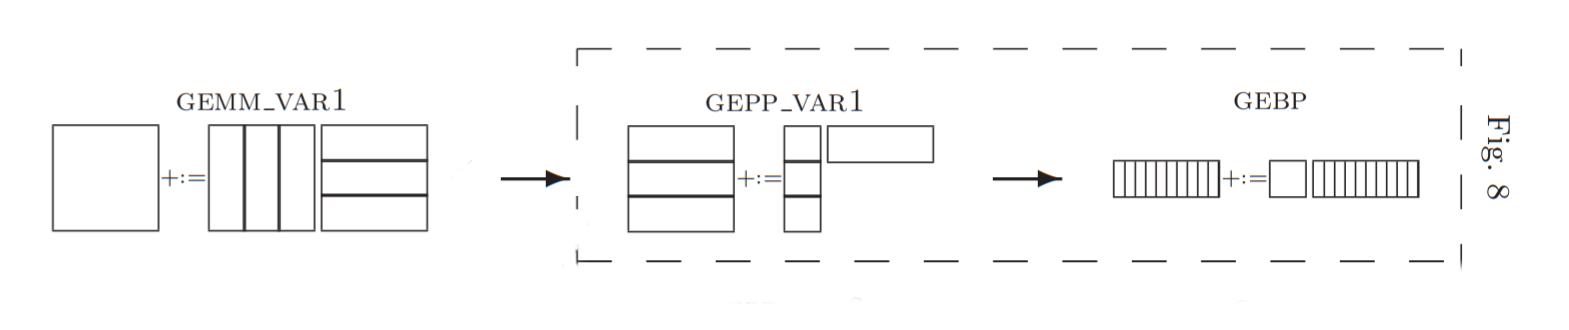
\includegraphics[width=\textwidth,height=6cm,keepaspectratio=true]{../figs/dgemm_goto1.png}
    \caption{Illustration of Fig.8 in the paper \cite{Goto08}}
    \label{fig:dgemm1}
\end{figure}

This implentation has additional optimisations compares to the Implementation 1. While we only do blocking in cache previously, in this implentation, we also do blocking at the register level. Besides, we did additional data packing so that data access is in the contiguous memory. 

Following the \ref{fig:dgemm1}, we implemented dgemm through 3 functions:
\begin{itemize}
  \item $dgemm\_opt()$: where we splitted the matrix A and B to vertical panels and horizontal panels, respectively. The resulted matrix C will the accumulated summation of $A_i*B_i$.
  \item $gepp()$: this function performs a vertical panel $A_i$ by horizontal panel $B_i$ multiplication. We splitted the verticle panel further into blocks $A_{ij}$. Each horizontal panel $C_j$ will be the result of $A_{ij} * B_i$.
  \item $gebp()$: this function performs a block by horizontal panel multiplication. The horizontal panel $B_i$ and $C_j$ can be splitted further into vertical panels. With this, the $C_{jk}$ panel will be the result of $A_{ij}*B_{ik}$. One should try to fit the block $A_{ij}$ and panels $C_{ik}$, $B_{ik}$ into either L1 cache, or the size of TLB table. The Illustration for $gebp$ can be found at \ref{fig:dgemm2}
  Further decomposition of these block and panels can be performed so that the accessing data is fitted into registers, illustrated at \ref{fig:gebp}.  
\end{itemize}
\begin{figure}[htpb]
    \centering
    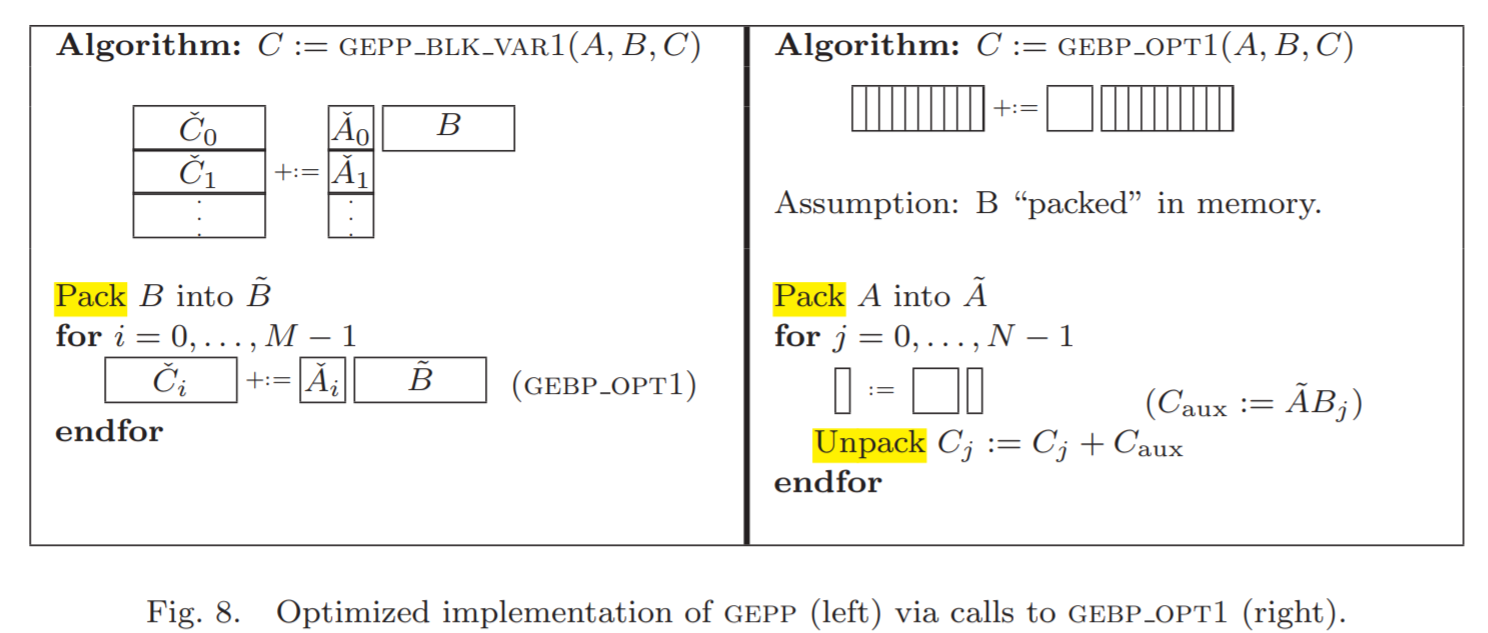
\includegraphics[width=\textwidth,height=6cm,keepaspectratio=true]{../figs/dgemm_goto2.png}
    \caption{ Implementation description for Fig.8 from the paper \cite{Goto08}}
        \label{fig:dgemm2}
\end{figure}


\begin{figure}[htpb]
\centering
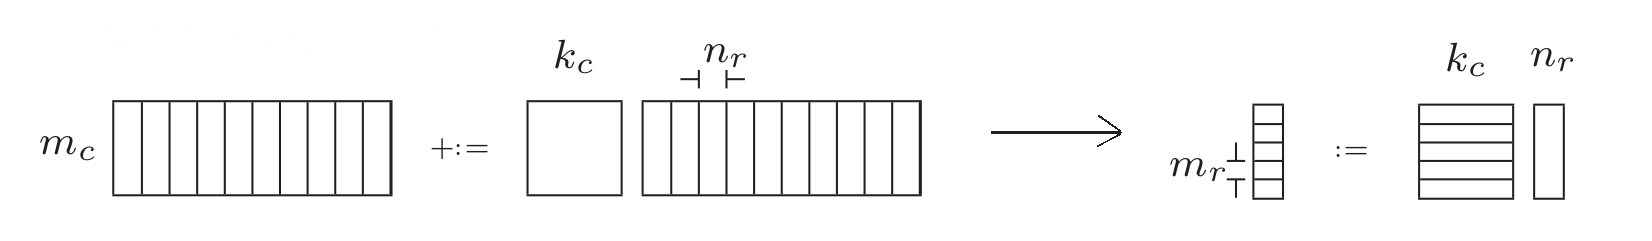
\includegraphics[width=\textwidth,height=6cm,keepaspectratio=true]{../figs/gebp.png}
\caption{ Illustration of further gebp decomposition.\cite{Goto08}}
\label{fig:gebp}
\end{figure}

\subsubsection{Additional Optimization}
Besides optimizations in the code, we also added additional optimisation through compiler flags. We replacted $-O3$ by $-Ofast$ to get further possible optimisation, and $-fargument-noalias -fno-alias$ tell the compiler that no aliasing is present globally.

\subsection{Results and Discussion}
Our best performance is with Implementation 2 which we referred from /cite{Goto08}. The best results are presented in the below table:

\begin{center}
	\begin{tabular}{|c |c c c c c c c|c| c| }
		\hline
		Node  & $K$   & $M$ & $N$    & $m_c$ & $k_c$ & $m_r$ & $n_r$ & $GFLOPs$ & $P/P_{peak}$  \\
		\hline
		Login & 128 & 32    & 32   &  32  & 32   & 32   & 2   & 27.13 & 65.2\% \\        
		Compute & 128 & 32    & 32   &  32  & 32   & 32   & 2   & 21.48 & 51.6\% \\        
		Login & 128 & 128    & 64   &  32  & 64   & 32   & 2   & 31.39 & 75.5\% \\         
		Compute & 128 & 128    & 64   &  32  & 64   & 32   & 2   & 24.75  & 59.5\%  \\
		\hline        
	\end{tabular}
\end{center}
For the dgemm with K=128, small M and N, we got the best performance for M=N=32. With these values, we have $m_c = k_c = 32$ which means the submatrix $A_{ij}$ has 1024 entries fitting perfectly into the TLB (Haswell has 1024 entries according to \cite{tlb}). Regarding the choice of $m_r$ and $n_r$, ideally $m_r*n_r$ should be half of number of available registers. However, we could not found out how many registers this CPU model has nor why the best values of $m_r$ and $n_r$ are larger than expected.\\

Even though the task requires M and N smaller than 32, we increased the value further for testing purpose, and got better performance. The choice of $m_c=64$ and $k_c=32$ makes $A_{ij}$ to have 2048 entries, which saturated half the L1d. This is the desired number according to \cite{Goto08}.\\

The performance varies from the login node to compute node which is quite surprising. Normally, one would expect to have better performance on compute node than login node since the resource is shared on the login node. We don't have a clear explanation for this.

\medskip
%\printbibliography
\bibliography{myref}{}
\bibliographystyle{plain}

\end{document}


